% Chapter Template

\chapter{Implementation} % Main chapter title

\label{Chapter5} % Change X to a consecutive number; for referencing this chapter elsewhere, use \ref{ChapterX}

\lhead{Chapter 5. \emph{Implementation}} % Change X to a consecutive number; this is for the header on each page - perhaps a shortened title

%----------------------------------------------------------------------------------------

\section{Introduction}

This chapter will discuss in detail, the implementation of the proposed android client application, and the server application that accompanies it.

With the system already designed out, I started exploring various coding patterns I could use to implement my design.

\subsection{Architecture and Design Patterns}

Design patterns are reusable solutions to commonly occurring problems in software design. The use of tried and tested design patterns is important in software because it stops programmers from making the same mistakes, and also speeds up development time as you no longer need to 'reinvent the wheel' with every software engineering project.

Picking the correct design pattern for the problem can prove troublesome, and choosing the wrong ones can lead to inefficient solutions, such as unnecessary duplication of code.

For this project, MVC was used heavily in both the client and server side application.

\subsection{Model-View-Controller (MVC)}

Model-View-Controller is a well known software design pattern for implementing user interfaces. The design follows three interconnected parts:

\begin{itemize}
	\item Model - holds the application data, and logic  for accessing and manipulating this data.
	\item View - holds logic that displays the aesthetic view to the user. It can also contain mechanisms of receiving user input and passing that input along to it's controller.
	\item Controller - holds controller logic that accesses data from a model and passes it to a view. It can also update a models state with new information, and update the view as the model is updated.
\end{itemize}

Figure \ref{fig:mvc} shows the MVC architecture.

\begin{figure}[htbp]
	\centering
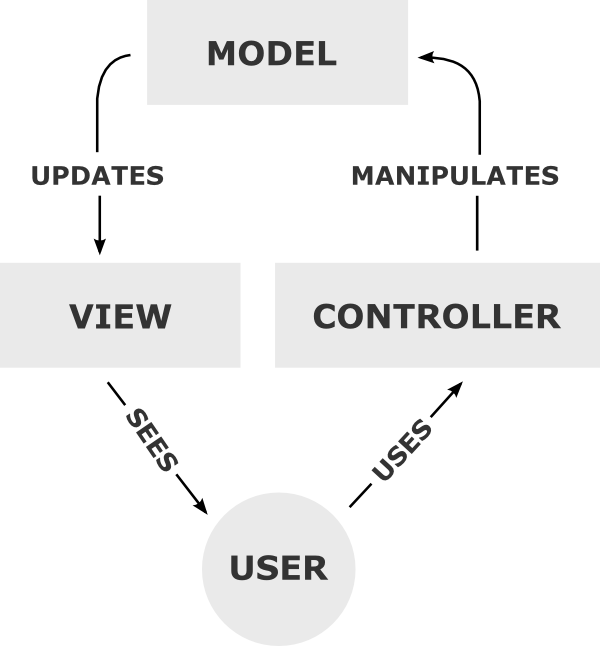
\includegraphics[width=10cm,height=10cm,keepaspectratio]{Figures/MVC.png}	
		\rule{35em}{0.5pt}
	\caption[Model View Controller Diagram - \cite{wikiMVC}]{Model View Controller Diagram - \cite{wikiMVC}}
	\label{fig:mvc}
\end{figure}

The server application makes heavy use of certain aspects of MVC. Models are created for data storage and the transport of the objects from server to client. Controllers are also created to design restful web requests that the client can use to request the data models remotely. Views are not used in the project because no user interface is required for the web server.

The android client application also uses this pattern, with the controllers requesting data from the remote server, using models to formulate the data into the right structure, and displaying the data in views.

\subsection{Data Transfer}

The data models are shared and used in both the client and the server. 

This makes data transfer incredibly easy; data can be de-serialised into a JSON format by the server, sent to the client, and then serialised back into the same object using the same model. 

This removes the need for duplicate code and removes any complications in the transfer process, such as parsing the JSON manually to determine the data structure.

\subsection{Asynchronous Requests}

A problem I encountered early on in the project's implementation was that while the client made requests, the program would halt until it received a response from the server (or the connection timed out). To solve this issue, I implemented asynchronous requests so that the program would continue functioning without waiting for a request to return its result first.

\subsection{User Interface and Storyboards}

\section{Server Implementation}
\subsection{Data Access Layer}
\subsection{Data Layer}
\subsection{Business Layer}
\subsection{Application Layer}

\section{Client Implementation}
\subsection{Data Access Layer}
\subsection{Data Layer}
\subsection{Business Layer}
\subsection{Application Layer}

%----------------------------------------------------------------------------------------